\documentclass{beamer}
\usepackage{listings}
\lstset{
%language=C,
frame=single, 
breaklines=true,
columns=fullflexible
}
\usepackage{subcaption}
\usepackage{url}
\usepackage{amsmath}

\usepackage{amsthm}

\usepackage{tikz}
\usepackage{graphicx}
\usepackage{tkz-euclide} % loads  TikZ and tkz-base
%\usetkzobj{all}
\usetikzlibrary{calc,math}
\usepackage{float}

\newcommand\norm[1]{\left\lVert#1\right\rVert}
\renewcommand{\vec}[1]{\mathbf{#1}}
\newcommand{\R}{\mathbb{R}}
\newcommand{\C}{\mathbb{C}}
\providecommand{\brak}[1]{\ensuremath{\left(#1\right)}}
\providecommand{\abs}[1]{\vert#1\vert}
\providecommand{\fourier}{\overset{\mathcal{F}}{ \rightleftharpoons}}
\newcommand{\myvec}[1]{\ensuremath{\begin{pmatrix}#1\end{pmatrix}}}
\providecommand{\mean}[1]{E[ #1 ]}
\providecommand{\sbrak}[1]{\ensuremath{{}\left[#1\right]}}
\providecommand{\cbrak}[1]{\ensuremath{\left\{#1\right\}}}
\usepackage[export]{adjustbox}
\usepackage[utf8]{inputenc}
\usepackage{amsmath}
\usetheme{Boadilla}
\title{GATE 2021 EC Q4}
\author{Adepu Adarsh Sai}
\institute{IITH(AI)}
\date{\today}
\begin{document}

\begin{frame}
\titlepage
\end{frame}
\begin{frame}{Dirac-delta Impulse}
    \begin{block}{Dirac-delta Impulse}
    \begin{align}
 \delta\brak{t}=
 \begin{cases}
 \infty , & t=0\\
 0, & otherwise
 \end{cases}
\end{align}
    \end{block}
\begin{block}{Shifting property of $\delta\brak{t}$}
If $g\brak{t}$ is a continuous and finite function at $t=a$ then
 \begin{align}
     \int_{-\infty}^{\infty}\delta\brak{t-a}g\brak{t}dt=g\brak{a}
 \end{align}
\end{block}
\end{frame}
\begin{frame}{}
    \begin{block}{Theorem-1}
      Fourier transform of shifted impulse is the complex exponential.
\begin{align}
    G\brak{f}=\mathcal{F}\cbrak{\delta\brak{t-a}}=e^{-i2\pi fa}
\end{align}
    \end{block}
    \begin{block}{Proof}
      \begin{align}
     G\brak{f}&=\int_{-\infty}^{\infty}\delta\brak{t-a}e^{-i2\pi ft}dt\\
     &=e^{-i2\pi fa}
 \end{align}
    \end{block}
\end{frame}
\begin{frame}
     \begin{block}{Corollary-1}
      Inverse Fourier Transform of the complex exponential must be the shifted impulse. So
\begin{align}
    \mathcal{F}^{-1}\cbrak{e^{-2\pi fa}}&=\int_{-\infty}^{\infty}e^{-2\pi fa}e^{i2\pi ft}df\\
    &=\int_{-\infty}^{\infty}e^{i2\pi f\brak{t-a}}df\\
    &=\int_{-\infty}^{\infty}e^{-i2\pi f\brak{t-a}}df\\
    \implies \int_{-\infty}^{\infty}e^{-i2\pi f\brak{t-a}}df &=\delta\brak{t-a}
\end{align}
    \end{block}
\end{frame}
\begin{frame}{}
    \begin{block}{Theorem-2}
     The Fourier transform of $g\brak{t}=e^{i2\pi at}$ is given by 
\begin{align}
    G\brak{f}=\mathcal{F}\cbrak{e^{i2\pi at}}=\delta\brak{f-a}
\end{align}
    \end{block}
    \begin{block}{Proof}
     \begin{align}
     G\brak{f}&=\int_{-\infty}^{\infty}e^{i2\pi at}e^{-i2\pi ft}dt\\
     &=\int_{-\infty}^{\infty}e^{i2\pi t\brak{a-f}}dt\\
     &=\delta\brak{f-a}
 \end{align}
    \end{block}
\end{frame}
\begin{frame}{}
  \begin{block}{Linearity of Fourier Transform}
   \begin{align}
    \mathcal{F}\cbrak{c_1g\brak{t}+c_2h\brak{t}}=c_1\mathcal{F}\cbrak{g\brak{t}}+c_2\mathcal{F}\cbrak{h\brak{t}}
\end{align}
  \end{block} 
  \begin{block}{Lemma-1}
   Let $x\brak{t}$ be a signal, its Fourier Transform  be of the form
\begin{align}
    G_x\brak{f}=c_1\delta\brak{f-a_1A}+c_2\delta\brak{f-a_2A}+...
\end{align}
where $c_i\in \mathbb{C}$ and $a_i\in \mathbb{R}$. 
Then the frequencies present in the signal are $a_jA $ where $a_j\in \mathbb{R}^{+}$
  \end{block}
\end{frame}
\begin{frame}{Fourier Transform of Cosine function}
    Let $x\brak{t}=\cos{\brak{2\pi At}}$, where $A=10kHz$.
\begin{align}
  \cos{\brak{2\pi At}}=\frac{e^{i2\pi At}+e^{-i2\pi At}}{2}  
\end{align}
The Fourier transform of $x\brak{t}$ 
\begin{align}
    G_x\brak{f}&=\int_{-\infty}^{\infty}\frac{e^{i2\pi At}+e^{-i2\pi At}}{2}e^{-i2\pi ft}dt\\
    &=\frac{1}{2}\sbrak{\int_{-\infty}^{\infty}e^{-i2\pi t(f-A)}dt+\int_{-\infty}^{\infty}e^{-i2\pi t(A+F)}}\\
    &=\frac{1}{2}\sbrak{\delta\brak{f-A}+\delta\brak{f+A}}
\end{align}
$\therefore$ All the energy of the sinusoidal wave is  entirely localized at the frequencies given by $|f|=A$.
\end{frame}
\begin{frame}{Question}
 \begin{block}{Gate 2021 EC Q4}
  Consider a real-valued base-band signal $x\brak{t}$, band limited to 10 kHz. The Nyquist rate for the signal $y\brak{t} = x\brak{t}x\brak{1+\frac{t}{2}}$ is
\begin{enumerate}
    \item 15 kHz
    \item 30 kHz
    \item 60 kHz
    \item 20 kHz
\end{enumerate}
 \end{block}   
\end{frame}
\begin{frame}{Solution}
    \begin{align}
    y\brak{t}&=\cos{\brak{2\pi At}}\cos{\brak{2\pi A\brak{1+\frac{t}{2}}}}\\
    &=\cos{\brak{2\pi A+3\pi At}}+\cos{\brak{2\pi A-\pi At}}\\
    &=\cos{\brak{3\pi At}}+\cos{\brak{\pi At}}\label{yt}
\end{align}
Using the linearity of Fourier Transform. Fourier Transform of $y\brak{t}$ is given by
\begin{multline}
    G_y\brak{f}=\frac{1}{2}\sbrak{\delta\brak{f-\frac{3A}{2}}+\delta\brak{f+\frac{3A}{2}}}\\+\frac{1}{2}\sbrak{\delta\brak{f-\frac{A}{2}}+\delta\brak{f+\frac{A}{2}}}
\end{multline}
\end{frame}

\begin{frame}
\begin{align}
  x\brak{t}&=\cos{\brak{20k\pi t}}\\
    \text{bandwidth of } x\brak{t} &= 10 kHz  
\end{align}
 \begin{figure}[!h]
 \centering
 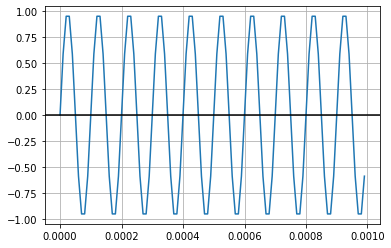
\includegraphics[width=0.6\textwidth]{x.png}
 \caption{$x\brak{t}$:Sinusoidal signal with freq=10kHz}
\end{figure}
\end{frame}
\begin{frame}
\begin{align}
     x\brak{1+\frac{t}{2}} &= \cos{\brak{20k\pi+10k\pi t}}\\
    \text{bandwidth of } x\brak{1+\frac{t}{2}} &=  5 kHz\\
    \text{from \eqref{yt} } 
    y\brak{t}&= \cos{\brak{30k\pi t}}+\cos{\brak{10k\pi t}}\\
    \text{bandwidth of } y\brak{t} &= \frac{30}{2} kHz\\
    &= 15 kHz
\end{align}
\begin{align}
    \text{Nyquist rate} &= 2 \times \text{maximum frequency}\\
    &= 30 kHz
\end{align} 
\end{frame}
\begin{frame}
    \begin{figure}[!h]
 \centering
 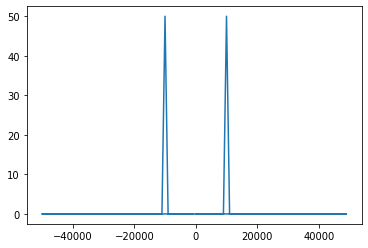
\includegraphics[width=0.6\textwidth]{xf.png}
 \caption{DFT of $x\brak{t}$. $Bandwidth=10000$}
\end{figure}
\end{frame}
\begin{frame}
   \begin{figure}[!h]
 \centering
 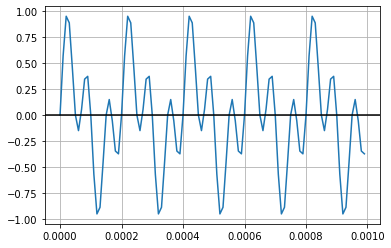
\includegraphics[width=0.4\textwidth]{y.png}
 \caption{$y\brak{t}$}
\end{figure}
\begin{figure}[!h]
 \centering
 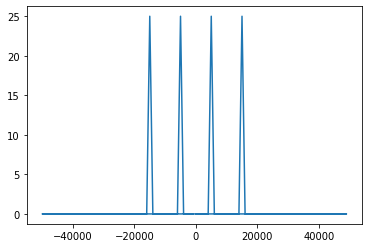
\includegraphics[width=0.4\textwidth]{f.png}
 \caption{DFT of $y\brak{t}$.$Bandwidth=15000$}
\end{figure} 
\end{frame}
\end{document}